% Source: PTZ, 140205, Latvia

\begin{problem}{Ship}{ship.in}{ship.out}{4 seconds}{32 mb}{}

A ship has been assigned to transport cargo across the river Daugava (Western Dvina) that has the capacity to carry at most $t$ tons of cargo. There is a hangar on the right bank of the river that contains $n$ cargo containers to be transported by the ship. The weight of each container is an integer number of tons and it does not exceed $t$ tons. The containers are arranged in a single line from the start to the end of the hangar. A container can be carried onto the ship by a liftloader that can pick only a container either at the start or at the end of the line. The total weight of the containers placed on a ship cannot exceed the capacity of the ship. None of the containers are allowed to be opened, thus it is impossible to redistribute the cargo among the containers. It is also expensive to move the containers so once the container has been picked up by the liftloader, it is then directly carried onto the ship. Only then the liftloader can pick another container from the hangar. Once the ship is loaded, it can transport the containers to the left bank and return to the right bank empty.

Write a program that calculates the minimum possible number of trips the ship has to make to transport all of the containers to the left river bank!

\InputFile
The first line of input contains two integers $t$ and $n$ ($1 \leq t \leq 10^9$, $1 \leq n \leq 10^4$), the capacity of the ship and the number of containers in the hangar, accordingly. The next line contains $n$ integers, the weight of the containers in tons. The $i$-th number $w_i$ ($1 \leq w_i \leq t$) denotes the weight of the $i$-th container from the start of the hangar. On each line the numbers are separated by spaces.

\OutputFile
Output a single integer: the minimum possible trip number for the ship to transport all of the containers to the other river bank.

\Examples

\begin{example}
\exmp{10 12
1 5 4 4 1 8 9 7 2 2 3 2
}{5
}%
\end{example}

\Note
The following figure shows the remaining containers in the hangar before and after each trip in the given example.
\begin{center}
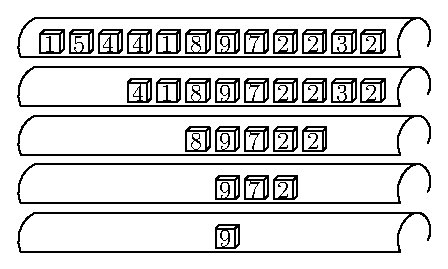
\includegraphics[bb = 60 0 140 120]{pics/figure.eps}
\end{center}

\end{problem}
